\documentclass[hints,nooutcomes,noauthor,handout,12pt]{ximera}

\graphicspath{  
{./}
{./whoAreYou/}
{./drawingWithTheTurtle/}
{./bisectionMethod/}
{./circles/}
{./anglesAndRightTriangles/}
{./lawOfSines/}
{./lawOfCosines/}
{./plotter/}
{./staircases/}
{./pitch/}
{./qualityControl/}
{./symmetry/}
{./nGonBlock/}
}


%% page layout
\usepackage[cm,headings]{fullpage}
\raggedright
\setlength\headheight{13.6pt}


%% fonts
\usepackage{euler}

\usepackage{FiraMono}
\renewcommand\familydefault{\ttdefault} 
\usepackage[defaultmathsizes]{mathastext}
\usepackage[htt]{hyphenat}

\usepackage[T1]{fontenc}
\usepackage[scaled=1]{FiraSans}

%\usepackage{wedn}
\usepackage{pbsi} %% Answer font


\usepackage{cancel} %% strike through in pitch/pitch.tex


%% \usepackage{ulem} %% 
%% \renewcommand{\ULthickness}{2pt}% changes underline thickness

\tikzset{>=stealth}

\usepackage{adjustbox}

\setcounter{titlenumber}{-1}

%% journal style
\makeatletter
\newcommand\journalstyle{%
  \def\activitystyle{activity-chapter}
  \def\maketitle{%
    \addtocounter{titlenumber}{1}%
                {\flushleft\small\sffamily\bfseries\@pretitle\par\vspace{-1.5em}}%
                {\flushleft\LARGE\sffamily\bfseries\thetitlenumber\hspace{1em}\@title \par }%
                {\vskip .6em\noindent\textit\theabstract\setcounter{question}{0}\setcounter{sectiontitlenumber}{0}}%
                    \par\vspace{2em}
                    \phantomsection\addcontentsline{toc}{section}{\thetitlenumber\hspace{1em}\textbf{\@title}}%
                     }}
\makeatother



%% thm like environments
\let\question\relax
\let\endquestion\relax

\newtheoremstyle{QuestionStyle}{\topsep}{\topsep}%%% space between body and thm
		{}                      %%% Thm body font
		{}                              %%% Indent amount (empty = no indent)
		{\bfseries}            %%% Thm head font
		{)}                              %%% Punctuation after thm head
		{ }                           %%% Space after thm head
		{\thmnumber{#2}\thmnote{ \bfseries(#3)}}%%% Thm head spec
\theoremstyle{QuestionStyle}
\newtheorem{question}{}



\let\freeResponse\relax
\let\endfreeResponse\relax

%% \newtheoremstyle{ResponseStyle}{\topsep}{\topsep}%%% space between body and thm
%% 		{\wedn\bfseries}                      %%% Thm body font
%% 		{}                              %%% Indent amount (empty = no indent)
%% 		{\wedn\bfseries}            %%% Thm head font
%% 		{}                              %%% Punctuation after thm head
%% 		{3ex}                           %%% Space after thm head
%% 		{\underline{\underline{\thmname{#1}}}}%%% Thm head spec
%% \theoremstyle{ResponseStyle}

\usepackage[tikz]{mdframed}
\mdfdefinestyle{ResponseStyle}{leftmargin=1cm,linecolor=black,roundcorner=5pt,
, font=\bsifamily,}%font=\wedn\bfseries\upshape,}


\ifhandout
\NewEnviron{freeResponse}{}
\else
%\newtheorem{freeResponse}{Response:}
\newenvironment{freeResponse}{\begin{mdframed}[style=ResponseStyle]}{\end{mdframed}}
\fi



%% attempting to automate outcomes.

%% \newwrite\outcomefile
%%   \immediate\openout\outcomefile=\jobname.oc
%% \renewcommand{\outcome}[1]{\edef\theoutcomes{\theoutcomes #1~}%
%% \immediate\write\outcomefile{\unexpanded{\outcome}{#1}}}

%% \newcommand{\outcomelist}{\begin{itemize}\theoutcomes\end{itemize}}

%% \NewEnviron{listOutcomes}{\small\sffamily
%% After answering the following questions, students should be able to:
%% \begin{itemize}
%% \BODY
%% \end{itemize}
%% }
\usepackage[tikz]{mdframed}
\mdfdefinestyle{OutcomeStyle}{leftmargin=2cm,rightmargin=2cm,linecolor=black,roundcorner=5pt,
, font=\small\sffamily,}%font=\wedn\bfseries\upshape,}
\newenvironment{listOutcomes}{\begin{mdframed}[style=OutcomeStyle]After answering the following questions, students should be able to:\begin{itemize}}{\end{itemize}\end{mdframed}}



%% my commands

\newcommand{\snap}{{\bfseries\itshape\textsf{Snap!}}}
\newcommand{\flavor}{\link[\snap]{https://snap.berkeley.edu/}}
\newcommand{\mooculus}{\textsf{\textbf{MOOC}\textnormal{\textsf{ULUS}}}}


\usepackage{tkz-euclide}
\tikzstyle geometryDiagrams=[rounded corners=.5pt,ultra thick,color=black]
\colorlet{penColor}{black} % Color of a curve in a plot



\ifhandout\newcommand{\mynewpage}{\newpage}\else\newcommand{\mynewpage}{}\fi

\title{Scaling roofs}


\author{Bart Snapp}

\begin{document}
\begin{abstract}
  Sometimes computing area is easy.
\end{abstract}
\maketitle


\begin{listOutcomes}
\item Apply the Pythagorean theorem to solve problems.
\item Extend ideas from two-dimensions to three-dimensions.
\item Follow steps in an algorithm to solve a problem.
\item Translate classroom mathematics into real world mathematics.
\item Recognize the difference between reasoning through formulas and
  reasoning through scaling.
\end{listOutcomes}


Imagine a house where the roof where two slopes meet. This will either
form a ``hip'' or a ``valley''.
\begin{center}
  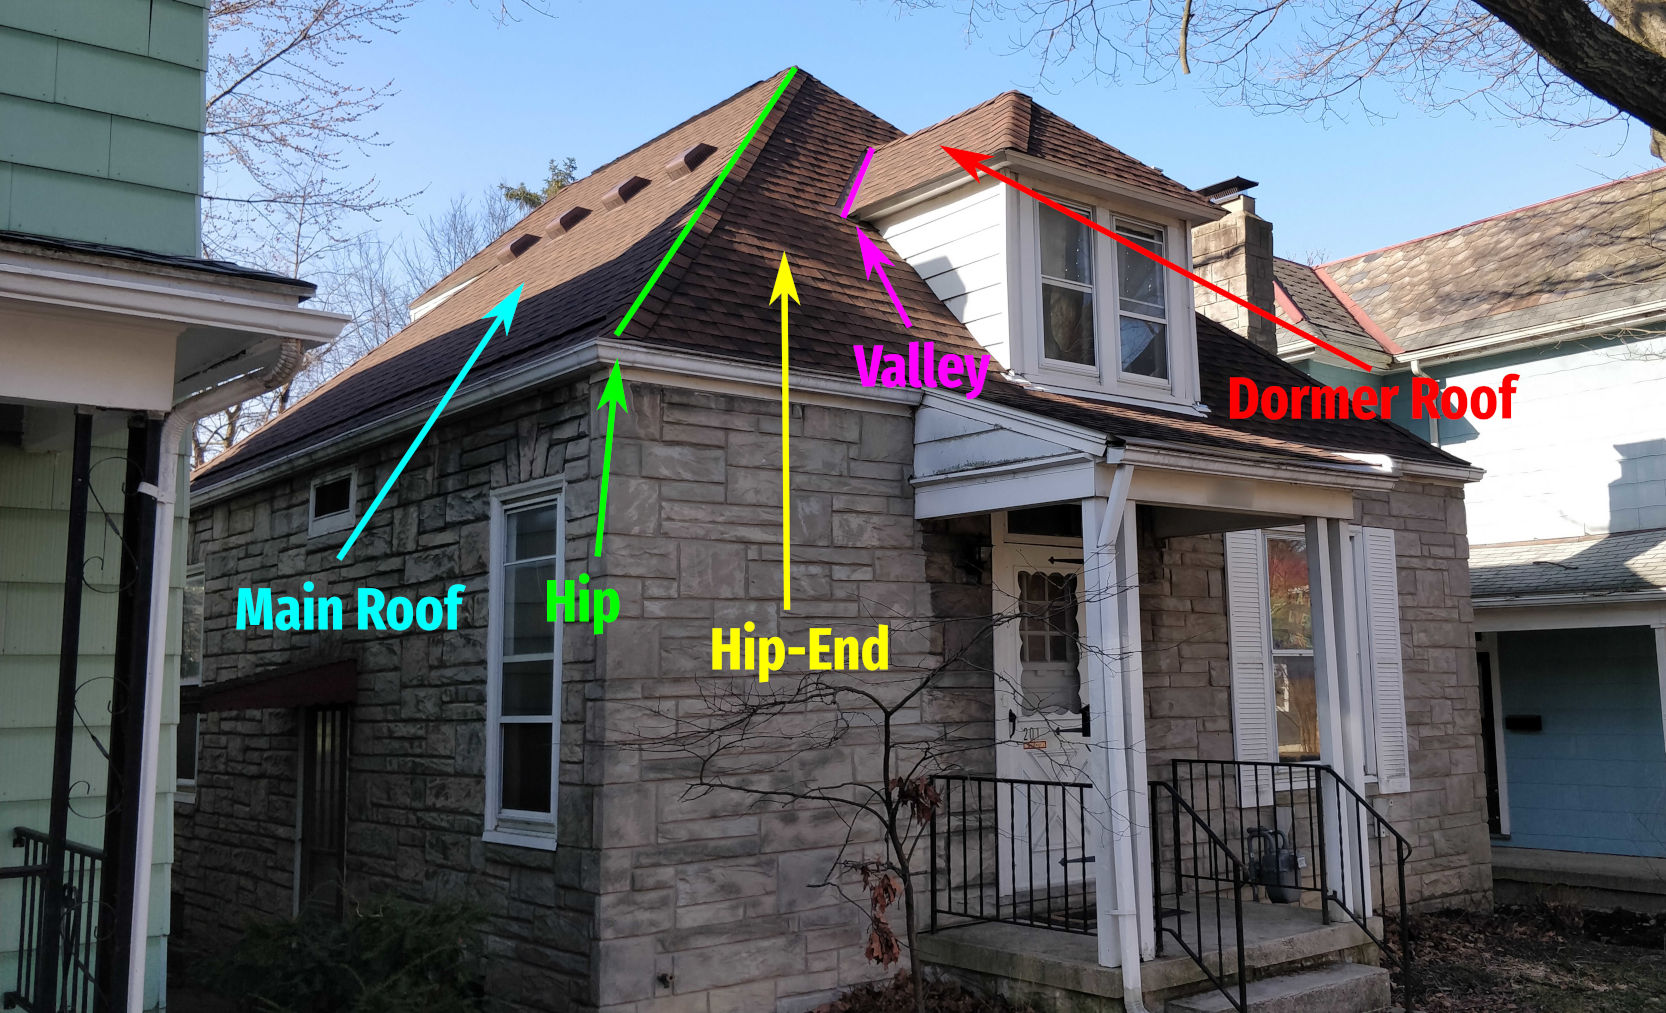
\includegraphics[width=.8\textwidth]{house.jpg}
\end{center}
Here's a question we want answered:
Given the dimensions (as seen from the top) of the roof, What is the AREA of the roof?



\mynewpage

\begin{question} We'll start by computing some areas.
\begin{enumerate}
\item Consider the \link[\textit{Luxor Las
    Vegas}]{https://en.wikipedia.org/wiki/Luxor_Las_Vegas}:
  \begin{center}
    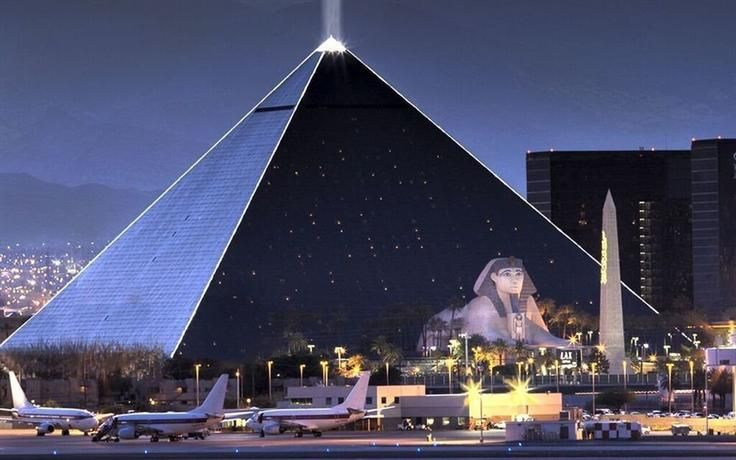
\includegraphics[width=.4\textwidth]{pyramid.jpg} 
  \end{center}
 Assuming that the (square) base of this building has a side length of
 $646$ feet and that the pyramid is $350$ feet tall, compute the
 surface in square feet, not including the bottom. Explain your
 reasoning and show your work.
\item Now imagine a different building with a square base of side
  length $646$, whose roof is a single plane at a slope of
  $\tfrac{350}{323}$. SKETCH a possible picture of this situation and
  find the AREA of this roof. Explain your reasoning and show your
  work.

\item Compare/contrast your answers from the parts above and discuss. 
\end{enumerate}
\end{question}
 
 \mynewpage
 
 \begin{question}
\begin{enumerate}
\item Here are plans for a $1$-car garage that I got from \link[\textit{Garage Plans by Behm Design}]{https://behmdesign.com/shop/}:
   \begin{center}
     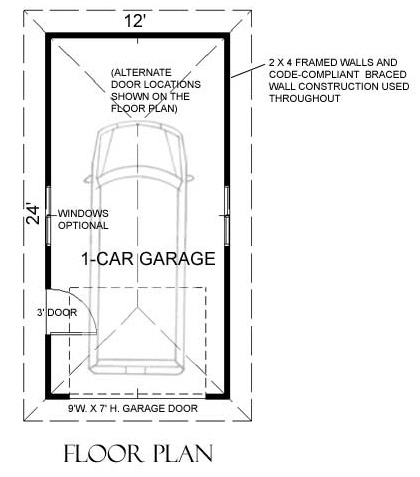
\includegraphics[width=.4\textwidth]{oneCarGarage.jpeg}
    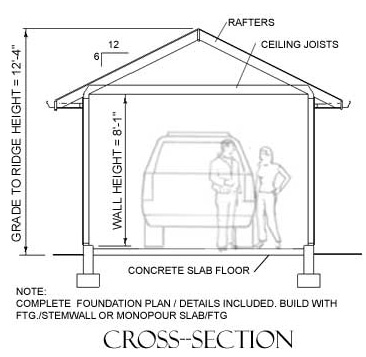
\includegraphics[width=.35\textwidth]{oneCarGarageFront.jpeg}
   \end{center}
   Assuming that the hip-end has a slope of $\frac{6}{12}$, and that
   the roof has an overhang of $2$ feet on all sides, find the area of
   the roof of the garage in square feet.  Explain your reasoning and
   show your work. %As a gesture of friendship, a 3D model is available
   %at: \url{https://www.geogebra.org/m/zu5zsvx6}
 \item Now suppose the building has a roof that is a single plane,
   covering a $16'$ foot by $28'$ rectangle that is at a slope of
   $\frac{6}{12}$. SKETCH a possible picture of this situation and
   find the AREA of the roof in this case. Explain your reasoning and
   show your work.
\item Compare/contrast your answers from the parts above and discuss. 
   
\end{enumerate}

\begin{freeResponse}
  \begin{enumerate}
    \item We must compute the height of one face of the pyramid. By
      the Pythagorean theorem, we have
      \[
      323^2 + 350^2 = h^2
      \]
      so
      \[
      h \approx 476.
      \]
      This means the top of the pyramid has a surface area of
      \[
      \text{Area} = 4\cdot \frac{646\cdot 476}{2} = 614992~\text{square feet}.
      \]
    \item Since there is an overhang of $2$ feet per side, the
      perimeter of the roof is a $16\times 28$ rectangle, meaning the
      area of the roof is AT LEAST $16\cdot 28 = 448$ square feet. If
      the main roof has a slope of $\frac{6}{12}$, it raises by
      \[
      8'\cdot \frac{6}{12}  = 4'
      \]
      This means that the height of both the main roof and the hip-end is
      \[
      \sqrt{8^2+4^2} = \sqrt{80} \approx 9~\text{feet}
      \]
      as measured along the roof. Moreover, we must move $8'$ in from
      the hip-end to achieve this height. Hence the length of the main
      ridge is
      \[
      28-8-8 = 12~\text{feet}.
      \]
      Thus the area of the roof is
      \[
      2\cdot \underbrace{\frac{16\cdot 9}{2}}_{\text{hip-end}} +
      2\left(\underbrace{2\cdot \frac{8\cdot 9}{2} + 12\cdot
        9}_{\text{main roof}}\right) = 504~\text{square feet}.
      \]
    \item Since there is an overhang of $2$ feet per side, the
      perimeter of the roof is a $16\times 28$ rectangle. If the main
      roof has a slope of $\frac{6}{12}$, it raises by
      \[
      8'\cdot \frac{6}{12}  = 4~\text{feet}
      \]
      Again, the height as measured along the main roof is
      \[
      \sqrt{8^2+4^2} = \sqrt{80}\approx 9~\text{feet}.
      \]
      Since the slope of the hip-end is $\frac{8}{12}$, and
      \begin{align*}
        x\cdot \frac{8}{12} &= 4\\
        x = \frac{12\cdot 4}{8}\\
        x = 6,
      \end{align*}
      thus must move $6'$ in from the hip-end to achieve this height.
      So the height of the hip-end (as measured along the roof) is
      \[
      \sqrt{6^2+4^2} = \sqrt{50} \approx 7~\text{feet}
      \]
      Finally, note that the length of the main ridge is
      \[
      28-6-6 = 16~\text{feet}.
      \]
      Thus the area of the roof is
      \[
      2\cdot \underbrace{\frac{16\cdot 7}{2}}_{\text{hip-end}} +
      2\left(\underbrace{2\cdot \frac{6\cdot 9}{2} + 16\cdot
        9}_{\text{main roof}}\right) = 508~\text{square feet}.
      \]
  \end{enumerate}
\end{freeResponse}


\end{question}
\mynewpage










\mynewpage


\begin{question}
  Now let's reflect on the content above a bit. If all the slopes of a
  roof are the same, say $p/12$, there is an ``easy'' method of
  finding the area of the roof using SCALING.
  \begin{enumerate}
    \item Discover this method, and demonstrate that it is correct by using
    it to give to solve Problem $2$, part $(a)$ above.
    \item Use your method to derive the formula for the surface area
      of a cone. 
  \end{enumerate}
  \begin{freeResponse}
  If the slope is $\frac{p}{12}$, we multiply the area of the roof (as
  seen from above) by setting $p = 6$ and writing
    \[
    \frac{\sqrt{6^2+12^2}}{12} \approx 1.125.
    \]
    check it out:
    \[
    16\cdot 28 \frac{\sqrt{6^2+12^2}}{12} \approx 16\cdot 28 \cdot 1.125 = 504.
    \]
    Mic drop.
  \end{freeResponse}
\end{question}

\end{document}
